\chapter{实验结果与分析}

\section{数据集介绍}

为了比较上文提出的两个算法模型,分别从推荐结果的准确性、和算法训练与结果查询返回效率两个方面分别进行了两组实验。%
因此需要设计两组实验分别从算法推荐准确性和性能两个方面进行验证。本文评估上述两个算法在两个来自真实%
应用上的数据集,这些数据集都包涵用户与物品产生交互的时间戳:
\textbf{MovieLens}:MovieLens\footnote{\url{https://grouplens.org/datasets/movielens/}}是%
用来对推荐模型进行评估的最流行的基准数据集,它是由GroupLens研究组织从MovieLens网站收集的关于用户%
对电影评分的数据集,其中主要的评分文件以“用户ID | 电影ID | 评分 | 时间戳”为一行的格式%
保存了某个用户在某时刻对某个电影做出的评分标准,按照数据量的大小不同,本文选用的MovieLens数据集有%
Movielens 100K和Movielens 1M。

\textbf{Yoochoose}:Yoochoose\footnote{\url{http://2015.recsyschallenge.com}}数据集是%
2015年推荐系统顶级会议RecSys举办的挑战赛RecSys Challenge 2015上公开使用的目标数据集。%
Yoochoose包含了一个在线电子商务网站在6个月时间内用户所有的点击会话流。%


% \begin{table}[htbp]
% \centering
% \caption{数据集}
% \label{tab:dataset}
% \begin{minipage}[t]{0.9\linewidth}
% \begin{tabular*}{\linewidth}{c @{\extracolsep{\fill}} c @{\extracolsep{\fill}} c
% @{\extracolsep{\fill}} c @{\extracolsep{\fill}} c }
% \toprule[1.5pt]
% {\hei 数据集} & {\hei 类型} & {\hei 语言}
%  & {\hei 数量}\\
% \midrule[1pt]
% WWW & 论文摘要 & 英文 &  1330\\
% KDD & 论文摘要 & 英文 &  755\\
% Hulth03 & 论文摘要 & 英文 & 500\\
% \bottomrule[1.5pt]
% \end{tabular*}
% \label{tab3}
% \end{minipage}
% \end{table}


\section{评价指标}
作为一个推荐模型,模型会对查询目标给出点击可能性最高的N个物品,对于本文提出的序列推荐形式,%
模型的输入是$t$时刻及其以前的用户点击物品序列,需要的模型输出目标是$t+1$时刻用户可能点击%
的物品,以$\hat{I}_{u}^{t+1}$表示,

在关键词抽取工作中,提出过很多评价方法,其中最为常用的是准确%
率(Precision)、召回率(Recall)、准确率和召回率的调和平均数F1值(F1-score和MRR,%
本文也选用这三种评价指标验证关键词抽取算法的有效性。

\textbf{准确率}又名查准率,本文中通过将算法自动抽取的关键词和人工标记的关键词进行交集运算,%
例如:同一篇论文摘要,算法自动抽取出的Top
4关键词集合为 $E(k) = \{"hfmd","EV71","a16","encephalitis"\}$,
人工标注的关键词集合为
$S(k) = \{"hfmd","enterovirus 71"," coxsackie virus","Picornaviridae"\}$, 两个集合的交集为\{“hfmd”\},所以正确抽取的关键词个数为1个。因此,准确率、召回率和F1值的公式~(\ref{equ:chap05:extP})~(\ref{equ:chap05:extR})~(\ref{equ:chap05:extF1})所示:
\begin{equation}
\label{equ:chap05:extP}
Precision = \frac{E(k) \cap S(k)}{E(k)}
\end{equation}
\begin{equation}
\label{equ:chap05:extR}
Recall = \frac{E(k) \cap S(k)}{S(k)}
\end{equation}
\begin{equation}
\label{equ:chap05:extF1}
F1-score = \frac{2*Precision*Recall}{Precision+Recall}
\end{equation}

\subsection{学者推荐评价指标}
在学者推荐实验中,我们在微软学术数据上进行实验,%
针对无标签数据,本文通过采用对比的方式进行结果%
评价,即将本模型的推荐结果与微软学%
术的推荐列表进行对比。该设计的灵感源自于关键词抽取的评价标准,将微软学术官网的学者推%
荐列表作为正确结果,当用户搜索关键词后,%
微软学术会根据搜索%
的关键词推荐相应的学者,因此本文在无标签的情况下,为了验证模型有效性,就通过与权威的结果进行比对%
以此证明实验的可行性。微软学术的推荐结果可能是综合考虑多%
项指标之后,例如文献的引用次数、下载量、影响因%
子,作者的影响力、发文数量等,本文是在仅仅只有%
文本数据,而没有其他相关指标的情况下设计的推荐%
模型。通过查阅文献还发现,部分学者也曾在文献中%
提出将自己算法的%
实验结果截图和比较权威的机构或者公司的结果截图%
作定性的对比,针对无标签的数据,该设计方案%
有一定的迁移意义。下图~\ref{fig:t2dm}左侧即为在微软学%
术官网搜索关键词"t2dm"(二型糖尿病)后推荐20个学者的列表%
,右侧为检索"t2dm"时相关的文献列表。本文%
取Top20、Top10、Top5三种结果,若本模型推荐%
的前10个学者中有6个在微软学术推荐的列表中出现,%
那么该模型的正确率为P(top10) = 6/10,召回率为R(top10) = 6/20。同理,若本模型推荐的前5个学者中有2个在微软学%
术推荐的列表中出现,那么该模型的正确率为%
P(top5) = 2/5,召回率为R(top5) = 2/20。
因此,学者推荐的评价公式
准确率、召回率和F1值的公式如~(\ref{equ:chap05:recomP})~(\ref{equ:chap05:recomR})~(\ref{equ:chap05:recomF1})所示:
\begin{equation}
\label{equ:chap05:recomP}
P = \frac{R(u) \cap T(u)}{R(u)}
\end{equation}
\begin{equation}
\label{equ:chap05:recomR}
R = \frac{R(u) \cap T(u)}{T(u)}
\end{equation}
\begin{equation}
\label{equ:chap05:recomF1}
F1-score = \frac{2*P*R}{P+R}
\end{equation}

\begin{figure}[htbp] % use float package if you want it here
  \centering
  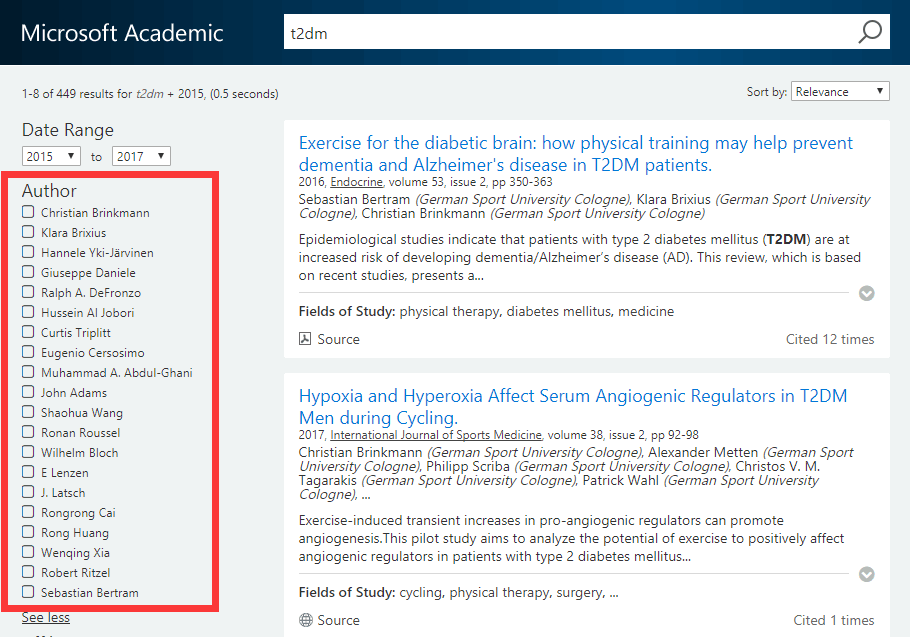
\includegraphics[width=\textwidth]{t2dm.png}
  \caption{红色方框列表则为在微软学术官网检索关键词“t2dm”时的推荐结果}
  \label{fig:t2dm}
\end{figure}

\section{实验结果与分析}

\subsection{关键词抽取结果}

\begin{table}[htbp]
\centering
\caption{关键词抽取准确率结果}
\label{tab:recommend}
\begin{minipage}[t]{0.9\linewidth}
\begin{tabular*}{\linewidth}{c @{\extracolsep{\fill}} c @{\extracolsep{\fill}} c @{\extracolsep{\fill}} c @{\extracolsep{\fill}} c @{\extracolsep{\fill}} c }
\toprule[1.5pt]
{\hei Dataset} & {\hei Method} & {\hei Top2}
 & {\hei Top4} & {\hei Top6} & {\hei Top8} \\
\midrule[1pt]
    & TF-IDF & 11.4 & 8.3 & 6.5 & 5.5 \\
KDD & TextRank & 9.5 & 8.1 & 7.1 & 6.3 \\
    & 融合后的算法 & 0.55 & 0.2 & 0.15 \\
\hline
    & TF-IDF & 12.2 & 9.1 & 7.0 & 5.8 \\
WWW & TextRank & 11.7 & 10.1 & 8.4 & 7.4 \\
    & 融合后的算法 & 0.55 & 0.2 & 0.15 \\
\hline
    & TF-IDF & 0.5 & 0.15 & 0.1 \\
Hulth03 & TextRank & 0.55 & 0.15 & 0.0 \\
    & 融合后的算法 & 0.55 & 0.2 & 0.15 \\
\bottomrule[1.5pt]
\end{tabular*}
\label{tab3}
\end{minipage}
\end{table}

\begin{table}[htbp]
\centering
\caption{关键词抽取召回率结果}
\label{tab:recommend}
\begin{minipage}[t]{0.9\linewidth}
\begin{tabular*}{\linewidth}{c @{\extracolsep{\fill}} c @{\extracolsep{\fill}} c @{\extracolsep{\fill}} c @{\extracolsep{\fill}} c @{\extracolsep{\fill}} c }
\toprule[1.5pt]
{\hei Dataset} & {\hei Method} & {\hei Top2}
 & {\hei Top4} & {\hei Top6} & {\hei Top8} \\
\midrule[1pt]
    & TF-IDF & 5.6 & 7.9 & 9.2 & 10.2 \\
KDD & TextRank & 4.6 & 7.7 & 9.9 & 11.8 \\
    & 融合后的算法 & 0.55 & 0.2 & 0.15 \\
\hline
    & TF-IDF & 5.4 & 7.3 & 8.4 & 9.2 \\
WWW & TextRank & 4.8 & 8.2 & 10.1 & 11.7 \\
    & 融合后的算法 & 0.55 & 0.2 & 0.15 \\
\hline
    & TF-IDF & 5.6 & 7.9 & 9.2 & 10.2 \\
Hulth03 & TextRank & 0.55 & 0.15 & 0.0 \\
    & 融合后的算法 & 0.55 & 0.2 & 0.15 \\
\bottomrule[1.5pt]
\end{tabular*}
\label{tab3}
\end{minipage}
\end{table}

\begin{table}[htbp]
\centering
\caption{关键词抽取F1-score结果}
\label{tab:recommend}
\begin{minipage}[t]{0.9\linewidth}
\begin{tabular*}{\linewidth}{c @{\extracolsep{\fill}} c @{\extracolsep{\fill}} c @{\extracolsep{\fill}} c @{\extracolsep{\fill}} c @{\extracolsep{\fill}} c }
\toprule[1.5pt]
{\hei Dataset} & {\hei Method} & {\hei Top2}
 & {\hei Top4} & {\hei Top6} & {\hei Top8} \\
\midrule[1pt]
& TF-IDF & 7.5 & 8.1 & 7.6 & 7.1 \\
KDD & TextRank & 6.2 & 7.9 & 8.3 & 8.2 \\
& 融合后的算法 & 0.55 & 0.2 & 0.15 \\
\hline
& TF-IDF & 7.1 & 8.1 & 7.7 & 7.1 \\
WWW & TextRank & 6.8 & 9.0 & 9.1 & 9.1 \\
& 融合后的算法 & 0.55 & 0.2 & 0.15 \\
\hline
& TF-IDF & 0.5 & 0.15 & 0.1 \\
Hulth03 & TextRank & 0.55 & 0.15 & 0.0 \\
& 融合后的算法 & 0.55 & 0.2 & 0.15 \\
\bottomrule[1.5pt]
\end{tabular*}
\label{tab3}
\end{minipage}
\end{table}

\subsection{学者推荐结果}

\begin{table}[htbp]
\centering
\caption{使用多种算法从关键词网络中选出核心节点的推荐结果表。}
\label{tab:recommend}
\begin{minipage}[t]{0.9\linewidth}
\begin{tabular*}{\linewidth}{c @{\extracolsep{\fill}} c @{\extracolsep{\fill}} c @{\extracolsep{\fill}} c @{\extracolsep{\fill}} c}
\toprule[1.5pt]
{\hei Dataset} & {\hei Method} & {\hei Top20}
 & {\hei Top10} & {\hei Top5} \\
 
\midrule[1pt]
& Degree Centrality & 0.5 & 0.15 & 0.1 \\

& Closeness Centrality & 0.55 & 0.15 & 0.0 \\

& Eigenvecter Centrality & 0.55 & 0.2 & 0.15 \\

HFMD & Jaccard & 0.4 & 0.35 & \textbf{0.25} \\

& Wang's method & \textbf{0.55} & \textbf{0.35} & 0.2 \\

& Liu's method & 0.45 & 0.25 & 0.0 \\

\hline
& Degree Centrality & 0.2 & 0.2 & 0.2 \\

& Closeness Centrality & 0.25 & 0.2 & 0.2 \\
 
& Eigenvecter Centrality & 0.2 & 0.0 & 0.0 \\
 
T2DM & Jaccard & 0.2 & 0.15 & 0.0 \\
 
& Wang's method & 0.2 & 0.0 & 0.0 \\
 
& Liu's method & \textbf{0.35} & \textbf{0.35} & \textbf{0.2} \\

\hline
 & Degree Centrality & 0.15 & 0.1 & 0.05 \\

& Closeness Centrality & 0.15 & 0.1 & 0.05 \\

& Eigenvecter Centrality & 0.15 & 0.1 & 0.05 \\

Pneumonia & Jaccard & \textbf{0.15} & \textbf{0.15} & \textbf{0.05} \\

& Wang's method & 0.15 & 0.1 & 0.05 \\

& Liu's method & 0.15 & 0.1 & 0.05 \\

\hline

 & Degree Centrality & 0.05 & 0.0 & 0.0 \\

& Closeness Centrality & 0.05 & 0.0 & 0.0 \\

& Eigenvecter Centrality & 0.05 & 0.05 & 0.05 \\

Cancer & Jaccard & \textbf{0.15} & \textbf{0.1} & 0.0 \\

& Wang's method & 0.05 & 0.05 & \textbf{0.05} \\

& Liu's method & -- & -- & -- \\
\bottomrule[1.5pt]
\end{tabular*}
\label{tab3}
\end{minipage}
\end{table}



\subsection{结果分析}

\section{本章小结}



